\chapter{Projektmanagement}
\label{pm-projektmanagement}
Hier finden Sie die Angaben zum Projekt, zu den eingesetzten Entwicklungs-Werkzeugen und zur eingesetzten Software.

\begin{itemize}
    \item Website: \url{http://play.kort.ch/} (\url{http://www.kort.ch/})
    \item Source Code: \url{https://github.com/kort/kort-reloaded/}
    \item Projektmanagement: Redmine (\url{sinv-56059.edu.hsr.ch/redmine/projects/ba-kort/ })
    \item Issues: (\url{http://sinv-56059.edu.hsr.ch/redmine/projects/ba-kort/issues}  (Backlog: im Wiki auf Redmine (mit SK für eigene Issues gekennzeichnet)) 
    \item Dokumentation: \url{https://github.com/kort/kort-reloaded-docu}
\end{itemize}

\section{Team}
\label{pm-rollen}
\begin{itemize}
	\item \textit{Betreuer}: Prof. Stefan F. Keller
	\item \textit{Projektpartner}: Liip AG, Limmatstrasse 183, CH-8005 Zürich
	\begin{itemize}
		\item Hr. Jürg Hunziker
		\item Hr. Stefan Oderbolz
	\end{itemize}
	\item \textit{Experte}: Hr. Claude Eisenhut
	\item \textit{Gegenleser}: Prof. Beat Stettler
\end{itemize}

\subsection*{Autoren}
Diese Arbeit wird als Bachelorarbeit an der Abteilung Informatik durchgeführt von
\begin{itemize}
	\item Hr. Marino Melchiori
	\item Hr. Dominic Mülhaupt
\end{itemize}


\section{Risikomanagement}
\label{pm-projektmanagement-risikomanagement}
Da \kort{} bereits in einer vorhergehenden Bachelorarbeit erfolgreich umgesetzt werden konnte und Anklang gefunden hat, wurden bereits viele Risiken abgedeckt.\newline
Dennoch wurde das Risikomanagement nicht vernachlässigt.
Alle bekannten Risiken sind gesammelt aufgelistet und wurden nach jedem Meilenstein neu evaluiert.

\subsection{Risikoanalyse}
\label{pm-projektmanagement-risikoanalyse}
Am Anfang der Bachelorarbeit wurden folgende Risiken identifiziert:

\begin{table}[H]
\centering
\label{pm-projektmanagement-risikomanagement-r01}
\begin{tabular}{|>{\raggedright}p{4.5cm}|p{11cm}|}
\hline
\multicolumn{2}{|l|}{\textbf{R01: Mangelnde Erfahrung mit \brand{JavaScript}, \brand{React} und \brand{React Native}}} \\
\hline
\textbf{Beschreibung} & Wirkt sich negativ auf Design und Programmcode aus. \\
\hline
\textbf{Schadenspotential} & 60h \\
\hline
\textbf{Eintrittswahrsch.} & 65\,\% \\
\hline
\textbf{Auswirkung} & Da die Entwickler sich mit den zugrundeliegenden Programmierkonzepten vertraut machen während sie bereits planen und Entscheidungen treffen, teilweise sogar schon programmieren müssen, kann und wird es vorkommen, dass gewisse Entscheidungen schlecht getroffen und gewisse Konzepte nicht sauber umgesetzt werden. 
Dies kann zu Verspätungen oder unsauberem Programmcode führen. \\
\hline
\textbf{Vorbeugung} & Die Entwickler haben mit dem Betreuer (Prof. Stefan Keller) besprochen, dass das \gls{Minimum Viable Product} der Bachelorarbeit eine Android App mit der gleichen Funktionalität, wie sie bereits im ursprünglichen Kort Game umgesetzt wurde, sein wird.
Im Rahmen dieser Arbeit blieb aber schlicht keine Zeit, um sich umfassend in die Technologien einzuarbeiten, bevor die restliche Arbeit angepackt ist.
Aus diesem Grund wird vor allem zu Beginn vermehrt auf \gls{Pair Programming} gesetzt.
Die Entwickler haben sich auch in regelmässigen Abständen die Zeit genommen, ein Code Review durchzuführen.
Ausserdem ist es wichtig, dass bei Schwierigkeiten nicht zu lange gezögert wird, den Kontakt zu Experten im jeweiligen Bereich zu suchen.  \\
\hline
\textbf{Massnahmen beim Eintreffen} & Komplexe Features vereinfachen und so gestalten, dass sie leicht erweiterbar sind. \\
\hline
\end{tabular}
\caption{Risiko R01}
\end{table}

\begin{table}[H]
\centering
\label{pm-projektmanagement-risikomanagement-r02}
\begin{tabular}{|>{\raggedright}p{4.5cm}|p{11cm}|}
\hline
\multicolumn{2}{|l|}{\textbf{R02: Es existiert keine passende Map Library für \brand{React Native}}} \\
\hline
\textbf{Schadenspotential} & 70h \\
\hline
\textbf{Eintrittswahrsch.} & 30\,\% \\
\hline
\textbf{Auswirkung} & Es müsste statt \brand{React Native} ein alternatives mobiles \gls{Framework} gefunden werden, welches die \brand{OSM}-Daten anzeigen kann. \\
\hline
\textbf{Vorbeugung} & Zu Beginn des Projektes muss eine \brand{React Native} Prototyp-Applikation implementiert werden, welche \brand{OSM}-Daten auf der Karte darstellt.  \\
\hline
\textbf{Massnahmen beim Eintreffen} & Auf eine aufwendigere Variante der Kartendarstellung, die im Kapitel \hyperref[tb-evaluation-karte]{Evaluation} evaluiert wurde, zurückgreifen. \\
\hline
\end{tabular}
\caption{Risiko R02}
\end{table}

\begin{table}[H]
\centering
\label{pm-projektmanagement-risikomanagement-r03}
\begin{tabular}{|>{\raggedright}p{4.5cm}|p{11cm}|}
\hline
\multicolumn{2}{|l|}{\textbf{R03: \brand{KeepRight} stellt den Dienst ein}} \\
\hline
\textbf{Schadenspotential} & 70h \\
\hline
\textbf{Eintrittswahrsch.} & 10\,\% \\
\hline
\textbf{Auswirkung} & Die Anzahl der zur Verfügung stehenden Missionen würde stark eingeschränkt werden.
Ausserdem wären diese auf die Schweiz beschränkt.
Ein anderer Dienst (z.\,B. \brand{Osmose}) müsste eingesetzt werden, was vor allem Änderungen im Backend erfordern würde. \\
\hline
\textbf{Vorbeugung} & Bereits früh im Projekt wird das Thema mit dem \hyperref[pm-team]{Projektpartner} besprochen, um festzustellen, ob dieser bereit wäre, sich dieser Problematik anzunehmen. \\
\hline
\textbf{Massnahmen beim Eintreffen} & Ausarbeitung einer neuen Aufgabenstellung mit dem Betreuer und den Projektpartnern (Jürg Hunziker und Stefan Oderbolz), die Änderungen am Backend beinhaltet. \\
\hline
\end{tabular}
\caption{Risiko R03}
\end{table}

\begin{table}[H]
\centering
\label{pm-projektmanagement-risikomanagement-r04}
\begin{tabular}{|>{\raggedright}p{4.5cm}|p{11cm}|}
\hline
\multicolumn{2}{|l|}{\textbf{R04: \brand{React Native} ist noch nicht ausgereift genug für \brand{Android}}} \\
\hline
\textbf{Schadenspotential} & 20h \\
\hline
\textbf{Eintrittswahrsch.} & 30\,\% \\
\hline
\textbf{Auswirkung} & \brand{Android} wird erst seit Oktober 2015 durch \brand{React Native} unterstützt. 
Einige Features von Komponenten stehen nur für \brand{iOS} zur Verfügung. \\
\hline
\textbf{Vorbeugung} & Bevor mit der Implementation begonnen wurde, sind die mangelnden Funktionalitäten (z.\,B. im Testing), so weit möglich, analysiert.
Grundsätzlich sollte es möglich sein, die App für \brand{Android} umzusetzen, da bereits komplexere Apps damit erstellt wurden.
Wahrscheinlich wird es vorkommen, dass Workarounds nötig sein werden. 
Im schlimmsten Fall müsste während der Entwicklung auf \brand{iOS} umgestellt werden, was grundsätzlich möglich ist. \\
\hline
\textbf{Massnahmen beim Eintreffen} & Ausarbeitung einer neuen Aufgabenstellung mit dem Betreuer, die eine \brand{iOS}-Version bevorzugt. \\
\hline
\end{tabular}
\caption{Risiko R04}
\end{table}

\begin{table}[H]
\centering
\label{pm-projektmanagement-risikomanagement-r05}
\begin{tabular}{|>{\raggedright}p{4.5cm}|p{11cm}|}
\hline
\multicolumn{2}{|l|}{\textbf{R05: Mangelnde Erfahrung mit der flux-Architektur}} \\
\hline
\textbf{Beschreibung} & Wirkt sich negativ auf Design und Programmcode aus. \\
\hline
\textbf{Schadenspotential} & 30h \\
\hline
\textbf{Eintrittswahrsch.} & 40\,\% \\
\hline
\textbf{Auswirkung} & Da die Konzepte der flux-Architektur neu erarbeitet werden müssen und flux in der Community als eher komplex eingestuft wird, kann die Entwicklung mehr Zeit beanspruchen. \\
\hline
\textbf{Vorbeugung} & Die korrekte Umsetzung wird bereits vor dem Start der Implementation so weit wie möglich analysiert.
Dabei wurden die Themengebiete zum Einlesen aufgeteilt und schlussendlich besprochen und erklärt. \\
\hline
\textbf{Massnahmen beim Eintreffen} & Rücksprache mit dem IFS-Team, das an einem \brand{React}-Projekt arbeitet. \\
\hline
\end{tabular}
\caption{Risiko R05}
\end{table}

\begin{table}[H]
\centering
\label{pm-projektmanagement-risikomanagement-r06}
\begin{tabular}{|>{\raggedright}p{4.5cm}|p{11cm}|}
\hline
\multicolumn{2}{|l|}{\textbf{R06: Mangelnde Erfahrung mit \gls{OAuth}}} \\
\hline
\textbf{Beschreibung} & Keiner der Entwickler ist mit \gls{OAuth} vertraut. Dadurch, dass sich die Implementation der Authentifizierung bei einem native Client zu einer Implementation einer \gls{WebApp} unterscheidet (Token- vs. Session-based), wird mehr Zeit beansprucht. \\
\hline
\textbf{Schadenspotential} & 40h \\
\hline
\textbf{Eintrittswahrsch.} & 60\,\% \\
\hline
\textbf{Auswirkung} & Die \brand{OSM}-Community würde nur sehr ungern auf einen entsprechenden Login verzichten. \\
\hline
\textbf{Vorbeugung} & Mehr Aufwand in die Evaluation stecken. \\
\hline
\textbf{Massnahmen beim Eintreffen} & Rücksprache mit dem Betreuer. \\
\hline
\end{tabular}
\caption{Risiko R06}
\end{table}

\subsubsection{Risikoanalyse MS2: Ende Elaboration -- 29.03.2016}
\textbf{R01: Mangelnde Erfahrung mit \brand{JavaScript}, \brand{React} und \brand{React Native}}: Die Eintrittswahrscheinlichkeit konnte auf 50\,\% gesenkt werden. 

\textbf{R03: \brand{KeepRight} stellt den Dienst ein}: Wurde nach Absprache mit den Projektpartnern (Jürg Hunziker und Stefan Oderbolz) ganz eliminiert.

\subsubsection{Risikoanalyse MS3: Evaluation der Komponenten -- 08.04.2016}
\textbf{R02: Es existiert keine passende Map Library für \brand{React Native}}: Die Wahrscheinlichkeit des Eintretens konnte nach erfolgreicher Implementation auf 20\,\% gesenkt werden. Dadurch, dass noch keine Missionen gelöst wurden, galt das Risiko noch nicht als behoben.

\subsubsection{Risikoanalyse MS4: Zwischenpräsentation -- 22.04.2016}
Das Eintreten von \textbf{R02} konnte weiterhin auf 10\,\% gesenkt werden. Die Marker waren klickbar und sie enthielten alle nötigen Informationen für das Lösen einer Mission.

\subsubsection{Risikoanalyse MS5: Basis-Komponenten umgesetzt -- 20.05.2016}
\textbf{R02} wurde eliminiert, \textbf{R01} auf 20\,\% gesenkt und \textbf{R05: Mangelnde Erfahrung mit der flux-Architektur} als tief eingeschätzt (10\,\%).

\subsubsection{Risikoanalyse MS6: Beta-Release mit Grundfunktionalität -- 06.06.2016}
\textbf{R05} wurde ebenfalls eliminiert -- die flux-Architektur war stabil und eine Mission konnte erfolgreich gelöst werden.

\subsubsection{Risikoanalyse MS7: Schlussabgabe -- 17.06.2016}
\textbf{R04: \brand{React Native} ist noch nicht ausgereift genug für \brand{Android}}: Wurde dank einer lauffähigen Version auf 10\,\% gesenkt.

\textbf{R06: Mangelnde Erfahrung mit OAuth}: Dies ist ein weiterhin bestehendes Risiko -- die \brand{OSM}-Authentifizierung konnte leider nicht umgesetzt werden.


\section{Projektplan}

\begin{figure}[H]
	\centering
	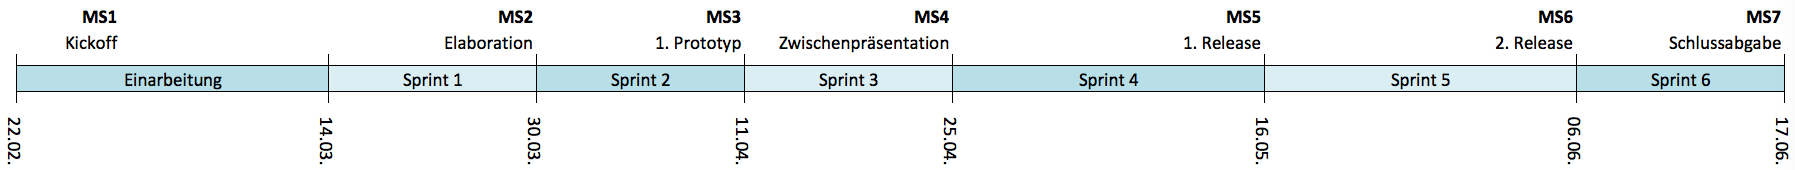
\includegraphics[width=\textwidth]{images/projektmanagement/zeitstrahl.png}
	\caption{Projektplan als Zeitstrahl dargestellt}
	\label{image-project-plan-timeline}
\end{figure}
% Anwendung von Scrum in unserem Projekt

\section{Meilensteine}
\label{pm-meilensteine}

In diesem Projekt wurde die Planung auf neun Meilensteine (MS) aufgeteilt. 
Die Meilensteine \hyperref[pm-ms8]{MS 8} und \hyperref[pm-ms9]{MS 9} finden nach der offiziellen Schlussabgabe statt und sind deswegen noch ohne Resultate dokumentiert.

\subsection{MS1: Kickoff}
\label{pm-ms1}
\textbf{Fällig am 25.02.2016}
\subsubsection{Resultate}
\begin{itemize}
	\item Kickoff Meeting bei Liip mit den Projektpartnern (Jürg Hunziker und Stefan Oderbolz) und dem Betreuer (Prof. Stefan Keller)
\end{itemize}

\subsection{MS2: Ende Elaboration}
\label{pm-ms2}
\textbf{Fällig am 29.03.2016}
\subsubsection{Resultate}
\begin{itemize}
	\item Infrastruktur aufgesetzt
	\begin{itemize}
		\item Datenbank
		\item \gls{CI}
		\item \brand{UserVoice}
		\item Redmine
		\item Installationsskripte
		\item Dokumentation aufgesetzt
	\end{itemize}
	\item Ausgangslage definiert und dokumentiert
	\item Anforderungsspezifikation erarbeitet
	\item Risikomanagement analysiert und dokumentiert
	\item Projektplan erarbeitet
	\item Map Komponente ausgewählt und eingesetzt
	\item Aufgabenstellung erarbeitet
	\item Testspezifikation erarbeitet
	\item Einarbeitung in die \kort{}-\gls{WebApp}
	\item \gls{GUI}-Mockups
\end{itemize}

\subsubsection{Erledigte Arbeiten}
Eine erste Version der Aufgabenstellung konnte erarbeitet werden. 
Die Dokumentation wurde eingeleitet.
Es gelang uns einen automatisierten Build der App aus dem \brand{GitHub}-Sourcecode mit \brand{Travis CI} aufzusetzen.
Für die Map-Komponente wurde die MapBox GL \gls{Library}\footnote{\url{https://libraries.io/npm/react-native-mapbox-gl}} mit den Vektor Daten von osm2vectortiles\footnote{\url{http://osm2vectortiles.org/}} evaluiert und getestet.
Nebenbei konnten wichtige Erfahrungen in den verwendeten Technologien (\brand{JavaScript}, \brand{React} und \brand{React Native}) gemacht werden.
Zusätzlich wurde ein für \brand{Android} angepasstes Design entworfen und Grundkonzepte der Architektur erarbeitet.
Die Architektur ist noch nicht final. 
Sie erleichtert uns aber den Einstieg beim Programmieren.
Die Infrastruktur ist soweit aufgesetzt.

\subsubsection{Probleme}
Für die detaillierte Erarbeitung der Testspezifikation fehlte noch die nötige Erfahrung in \brand{React Native}.


\subsection{MS3: Evaluation der Komponenten}
\label{pm-ms3}
\textbf{Fällig am 08.04.2016}
\subsubsection{Resultate}
\begin{itemize}
	\item Einarbeitung in \brand{JavaScript}, \brand{React} und \brand{React Native}
	\item \brand{Android} Prototyp
	\begin{itemize}
		\item Tab-Navigation
		\item Darstellung der Karte
		\item Evaluation der Architektur und Implementation des Grundgerüstes
		\item Missionen auf Map anzeigen
		\item Authentifizierung mit \gls{OAuth} evaluiert
	\end{itemize}
	\item \brand{Travis-CI} Konfiguration aktualisieren
\end{itemize}

\subsubsection{Erledigte Arbeiten}
Die Entwicklungsumgebung wurde optimiert. Das \brand{Travis}-Konfigurationsfile prüft den Code nun mit \brand{ESLint}\footnote{\url{http://eslint.org/}} (\brand{JavaScript} linter, prüft Styleguidelines) und \brand{flow}\footnote{\url{http://flowtype.org/}} (static type checker). 

Für die Tab-Navigation konnte eine Demo mit react-native-router-flux\footnote{\url{https://github.com/aksonov/react-native-router-flux}} umgesetzt werden. Diese muss noch in der \kort{} App implementiert werden. 

\gls{OAuth} (nur clientseitig, ohne Backend Kommunikation) wurde evaluiert und konnte dann anhand einer Demo getestet werden -- allerdings nur mit \brand{Facebook} und \brand{Google}.

Die Darstellung der Karte aus \nameref{pm-ms2} wurde leicht ausgebaut. Neu wird nun der Standort des Benutzers ermittelt.

Die Missionen konnten im Umkreis von fünf Kilometern geladen werden.

\subsubsection{Probleme}
Schwierigkeiten traten vor allem im Zusammenhang mit \brand{React Native} auf.
Oft gab es Build-Fehler bei gleicher Code-Basis.
Die Fehlerbehandlung hat uns enorm viel Zeit gekostet und es war schwer, im Internet Hilfestellungen zu erhalten.
Da \brand{React Native} alle zwei Wochen ein Update erhält, sind die Dokumentationen oder die Diskussionen im Internet teilweise schon wieder veraltet.\newline
Im Austausch mit anderen \brand{React Native} Entwicklern haben wir dasselbe Feedback erhalten.\newline
Der Prototyp konnte nicht wie geplant fertiggestellt werden und einige Arbeiten mussten auf den nächsten Meilenstein ausgelagert werden.

Die Authentifizierung mit dem Backend konnte noch nicht umgesetzt werden.

\subsection{MS4: Zwischenpräsentation}
\label{pm-ms4}
\textbf{Fällig am 22.04.2016}
\subsubsection{Resultate}
\begin{itemize}
	\item \brand{Mapbox} Prototyp fertig
	\begin{itemize}
		\item Missionen mit Marker auf Karte dargestellt
		\item Tab-Navigation implementiert
	\end{itemize}
	\item Zwischenpräsentation (Dauer ca. 30 Minuten)
	\begin{itemize}
		\item Aufgabenstellung, Problembesprechung
		\item IST-Situation
		\item geplantes Resultat
		\item Beschlussprotokoll für den \hyperref[pm-team]{Betreuer}
	\end{itemize}
\end{itemize}

\subsubsection{Erledigte Arbeiten}
Der Prototyp enthielt die Karte in einer Tab-Ansicht. 
An den jeweiligen Positionen der geladenen Missionen konnten Marker eingefügt werden.
Durch einen Klick auf einen Marker konnte der Titel der Mission erfolgreich in die Konsole geloggt werden.

Leider konnte noch immer keine Lösung für die Implementation eines Logins mit \gls{OAuth} 1.0a (\brand{OSM}) gefunden werden.
Dieses Feature noch zur Abgabe zu liefern wäre unrealistisch.
Deswegen wurde es auf den \hyperref[pm-ms9]{Meilenstein 9: Release für App Store} verschoben.

\subsubsection{Probleme}
Weiterhin traten Schwierigkeiten mit willkürlichen Fehlern der \brand{React Native} App auf. 
Aus diesen Gründen konnte die Navigation und die Struktur der App nicht abschliessend umgesetzt werden.
Dass der Benutzer nach dem Login automatisch zur Tab-Ansicht weitergeleitet wurde, hatte aufgrund eines Fehlers in der Navigations-\gls{Library} nicht geklappt.
Zwischenzeitlich wurde aus diesem Grund das Erhalten des Login-Tokens nach der Authentifizierung über \brand{Google} und \brand{Facebook} in einer separaten App getestet.


\subsection{MS5: Basis-Komponenten umgesetzt}
\label{pm-ms5}
\textbf{Fällig am 20.05.2016}
\subsubsection{Resultate}
\begin{itemize}
	\item Native Location Tracking implementiert
	\item \gls{GUI} fertig entworfen
	\item Testing-\gls{Framework} aufgesetzt
	\item Architektur-Entscheid und -Implementation
	\item Token basierte \brand{Google}-Authentifizierung im Frontend umgesetzt, nachdem das Backend vom Projektpartner, Stefan Oderbolz und Jürg Hunziker, dafür angepasst wurde
	\item \kort{}-Datenbank für Tests lokal aufgesetzt
	\item \kort{} ist \brand{iOS}-fähig
	\item \brand{React}-\gls{WebApp} evaluiert
	\item Validierungen vom Backend als Missionen laden
	\item Kurzvideo-Konzept besprochen
\end{itemize}

\subsubsection{Erledigte Arbeiten}

Wir haben die Architekturvarianten evaluiert und uns für die \brand{Flux}-Architektur entschieden.
Daraufhin wurde das bestehende -- noch sehr schlanke -- Grundgerüst, welches mit dem MVC-Pattern umgesetzt wurde, durch \brand{Flux} ersetzt.

Unterdessen konnte das Grundgerüst des \gls{GUI} grösstenteils fertiggestellt werden. 
Es fehlte noch die dynamische Behandlung von gewissen GUI-Komponenten.
Zum Beispiel die Unterscheidung, ob beim Lösen einer Mission ein Picker zum Auswählen der Antwort gerendert wird, oder ob ein Text-Input-Feld angeboten wird.

\kort{} konnte erfolgreich auf \brand{iOS} getestet werden. 

\subsubsection{Probleme}
Weiterhin war es nicht möglich mit der Router-Flux-Navigationskomponente eine Weiterleitung nach erfolgreichem Login zur Kartenansicht umzusetzen.
Hierbei handelte es sich um den bekannten Fehler dieser Komponente.
Das verzögerte leider das geplante Ziel: eine Mission zu lösen.

Die \kort{}-Datenbank konnte nur bei einem Entwickler richtig aufgesetzt werden. 
Es gab Probleme mit der Installation der Scripts auf \brand{OS X}.
Aus diesem Grund wurde für Tests nach Absprache mit dem Projektpartner (Jürg Hunziker), das Development-\kort{}-Backend genutzt.

\subsection{MS6: Beta-Release mit Grundfunktionalität}
\label{pm-ms6}
\textbf{Fällig am 06.06.2016}
\subsubsection{Resultate}
\begin{itemize}
	\item dynamische \gls{GUI} fertiggestellt
	\item Login Weiterleitung
	\item Login-Logik mit Local Storage
	\item Testing abgeschlossen
	\item Missionen und Validierungen sind lösbar
	\item Internationalisierung umgesetzt
\end{itemize}

\subsubsection{Erledigte Arbeiten}
Durch eine zusätzliche App-Loader-View konnte das Problem der Weiterleitung nach dem Login behoben werden.
Diese Komponente lädt nun alles im Voraus und erst danach wird je nach Zustand, ob der Benutzer eingeloggt ist oder nicht, die entsprechende Ansicht angezeigt.
Nach und nach wurden die Platzhalter der GUI mit dynamischen Daten der Businesslogik ersetzt. 
Die GUI ist nun dynamisch und zeigt je nach Zustand einer \inlinecode{Component} die entsprechende Oberfläche. 

Schlussendlich konnten wir erfolgreich Missionen und Validierungen lösen.


\subsubsection{Probleme}
Im \gls{Backend} sind Fehler aufgetreten wenn Validierungen negativ beantwortet wurden. 


\subsection{MS7: Schlussabgabe}
\label{pm-ms7}

\textbf{Fällig am 17.06.2016}

\subsubsection{Resultate}

\begin{itemize}
	\item Gebundene, vollständige Dokumentation eingereicht
	\item CD mit Abgabe eingereicht
	\item Abstract eingereicht
	\item Poster eingereicht
\end{itemize}


\subsection{MS8: Schlusspräsentation}
\label{pm-ms8}

\textbf{Fällig am 29.06.2016}

\subsubsection{Ziele}

\begin{itemize}
	\item Aktualisierte Dokumentation
	\item Design Verbesserungen
	\item Präsentation fertiggestellt
	\item Handouts ausgedruckt
\end{itemize}

\subsubsection{Resultate}

\begin{itemize}
	\item Dokumentation aktualisiert und neue CD gebrannt
	\item \brand{iOS} App getestet
\end{itemize}

\subsubsection{Probleme}
Bei der \brand{iOS} App funktioniert der Login mit \brand{Google} noch nicht. 
Es liegt ein Problem mit dem erhaltenen Token von \brand{Google} vor.

\subsection{MS9: Release für App Store}
\label{pm-ms9}

\textbf{Fällig am 05.07.2016}

\subsubsection{Ziele}

\begin{itemize}
	\item \brand{Android} App im \brand{Google Play} Store veröffentlicht
\end{itemize}
